\ifdefined\ishandout
\documentclass[handout]{beamer}
\else
\documentclass{beamer}
\fi

\usepackage[frenchb]{babel}
\usepackage[T1]{fontenc}
\usepackage[latin1]{inputenc}
\usepackage{hyperref}
\usepackage{multirow}
\usepackage{listings}
\usepackage{fancyvrb}
\usepackage{tikz}
\usepackage{framed}
\usepackage{algorithm}
\usepackage{algorithmic}
\usepackage{xcolor}
\usepackage{color, colortbl}
\usepackage{handoutWithNotes}

\usetikzlibrary{shapes.geometric}
\usetikzlibrary{positioning}
\usetikzlibrary{shapes.arrows, chains}
\usetikzlibrary{arrows,calc}
\usepackage{array}
\usetheme{Boadilla}

\ifdefined\ishandout
\pgfpagesuselayout{3 on 1 with notes}[a4paper,border shrink=5mm]
\usecolortheme{dove}
\else
\usecolortheme{dolphin}
\fi


\lstnewenvironment{codeC}
{ \lstset{language=C,
    otherkeywords={printf,scanf}}
}
{}

\ifdefined\ishandout
\definecolor{mygreen}{rgb}{0,0,0}
\definecolor{mymauve}{rgb}{0,0,0}
\definecolor{myblue}{rgb}{0,0,0}
\else
\definecolor{mygreen}{rgb}{0,0.6,0}
\definecolor{mymauve}{rgb}{0.58,0,0.82}
\definecolor{myblue}{rgb}{0,0,1}

\fi

\definecolor{mygray}{rgb}{0.5,0.5,0.5}


\lstset{language=C,
% breakatwhitespace=false,         % sets if automatic breaks should only happen at whitespace
%  breaklines=true,                 % sets automatic line breaking
%  captionpos=b,                
commentstyle=\itshape\color{mymauve},
keywordstyle=\bfseries\color{myblue},
%numbers=left,                    % where to put the line-numbers; possible values are (none, left, right)
%  numbersep=8pt,                   % how far the line-numbers are from the code
%  numberstyle=\tiny\color{mygray}, % the style that is used for the line-numbers
  rulecolor=\color{black},         % if not set, the frame-color may be changed on line-breaks within not-black text (e.g. comments (green here))
%  showspaces=false,                % show spaces everywhere adding particular underscores; it overrides 'showstringspaces'
  showstringspaces=false,          % underline spaces within strings only
%  showtabs=false,                  % show tabs within strings adding particular underscores
%  stepnumber=2,                    % the step between two line-numbers. If it's 1, each line will be numbered
  stringstyle=\color{mygreen},     % string literal style
%  tabsize=2 
}

\newcommand{\red}{\textcolor{red}}
%\newcommand \emph
%Default size : 12.8 cm * 9.6 cm

\newcommand{\tmark}[1]{\tikz[remember picture, baseline=-.5ex]{\coordinate(#1)}}

\ifdefined\ishandout
\newenvironment<>{codeblock}[1]{%begin
  \setbeamercolor{block title}{fg=black,bg=lightgray!80}%
  \begin{block}{#1}}
  % \begin{codeC}}
  %  {\end{codeC}
{  
\end{block}}

\newenvironment<>{termblock}[1]{
    \setbeamercolor{block title}{fg=black,bg=lightgray!90}%
    \begin{block}{#1}
}
%     \begin{Verbatim}}
{%\end{Verbatim}
\end{block}
}

\definecolor{bluegreen}{RGB}{0,0,0}
%\definecolor{bluegreen}{rgb}{0,0.6,0.8}
\else

\newenvironment<>{codeblock}[1]{%begin
  \setbeamercolor{block title}{fg=darkgray,bg=yellow}%
  \begin{block}{#1}}
  % \begin{codeC}}
  %  {\end{codeC}
{  
\end{block}}

\newenvironment<>{termblock}[1]{
    \setbeamercolor{block title}{fg=white,bg=lightgray}%
    \begin{block}{#1}}
%     \begin{Verbatim}}
{%\end{Verbatim}
\end{block}
}

\definecolor{bluegreen}{RGB}{0,149,182}
%\definecolor{bluegreen}{rgb}{0,0.6,0.8}
\fi

%\newcommand{\output}[1]{
\setbeamertemplate{navigation symbols}{}
\newcommand{\bvrb}{\Verb[commandchars=���,formatcom=\color{bluegreen}]}
\newcommand{\footvrb}{\footnotesize\Verb}


%%% Param�tres du cours (� r�gler)
%Num�ro du cours
\newcommand{\nb}{6}

\title[Cours n�\nb]{Cours n�\nb - Structures de donn�es - d�buggage}
\author[]{julien.brajard@upmc.fr}
\institute[Polytech' UPMC]{Polytech' UPMC}
\date{09 Novembre 2015}
\begin{document}
%%%%%%%%%%%%%%%%%%%%% SLIDES DE TITRE
\begin{frame}
\titlepage
\centering{
\url{http://australe.upmc.fr} (onglet EPU-C5-IGE Info Gen)}
\end{frame}
%%%%%%%%%%%%%%%%%%%%%
\begin{frame}
\frametitle{Plan du cours n�\nb}
\tableofcontents[hideallsubsections]
\end{frame}

%%%%



%%%%%% SECTION 12
% !TEX encoding = IsoLatin9
\section{Structures de donn�es}
\subsection{Introduction}
\begin{frame}
  \begin{columns}
    \column{4.8cm}
    \tableofcontents[currentsection,hideothersubsections,currentsubsection]
    \column{7cm}
    \centering{
      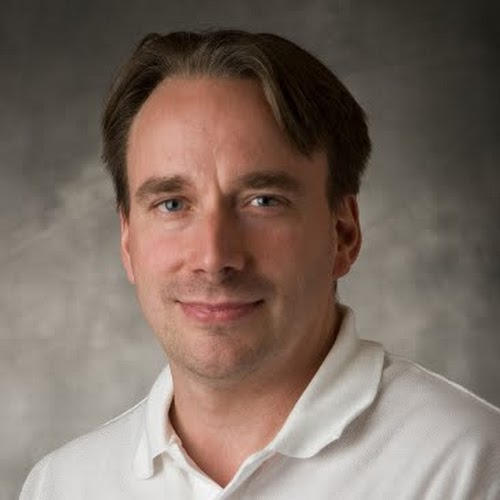
\includegraphics[width=4cm]{fig/linus.jpeg}
      }

      \textit{"I will, in fact, claim that the difference between a bad 
programmer and a good one is whether he considers his code or 
his data structures more important. Bad programmers worry 
about the code. Good programmers worry about data structures 
and their relationships."}\\
      \small{
        \hfill Linus Torvalds (1969-)\\
               \hfill cr�ateur de Linux}
    
  \end{columns}
  \end{frame}

\begin{frame}
\frametitle{D�finition}
\begin{block}{}
Une structure est un type de don�nes compos� de plusieurs
el�ments de type quelconque appel�s champs ou membres.
\end{block}
Les structures permettent de regrouper des informations
de types distincts mais ayant un lien s�mentique fort pour
le programmeur.
\begin{itemize}
\item Nom, Pr�nom, Date, lieu de naissance, adresse $\rightarrow$ \textbf{Identit�}
\item Jour, Mois, Ann�e $\rightarrow$ \textbf{Date}
\item Abscisse, Ordonn�e $\rightarrow$ \textbf{Point}
\end{itemize}

\begin{exampleblock}{Notes}
\begin{itemize}
\item Les structures compl�tent la notion de tableau car il devient
possible de regrouper des �l�ments de types diff�rents.
\item Les fonctions en C peuvent renvoyer une structure.
\end{itemize}

\end{exampleblock}

\end{frame}

\begin{frame}[fragile]
\frametitle{D�claration et initialisation}
Un mod�le de structure se d�fini de la fa�on suivante :
\begin{columns}
\column{.25\textwidth}
\begin{figure}
\begin{tikzpicture} [
auto,
remember picture,
 block/.style    = { rectangle, draw=blue, black, 
                         text width=2.8cm, text centered,
                         font = \footnotesize,
                        rounded corners, minimum height=2em },
node distance=0.5em,
]
\node (etiq) [block] {Etiquette de structure};
\node (point) [block, below= of etiq.south, anchor = north] 
{D�claration et initialisation d'un pointeur sur \bvrb|struct point|};

\end{tikzpicture}
\end{figure}
\column{.44\textwidth}

\begin{codeblock}{}
\vspace{-.3cm}
\lstset{escapeinside={��}}
\lstset{basicstyle=\scriptsize}
\begin{codeC}
struct �\tmark{c_etiq}�point {
 float x;�\tmark{c_champ1}�
 float y;�\tmark{c_champ2}�
 char couleur[10];�\tmark{c_champ3}�
};

struct point p1={1,-2,"Vert"};�\tmark{c_val}�

�\tmark{c_point1}�struct point * Ptr_point;
�\tmark{c_point2}�Ptr_point=&p1;
\end{codeC}
\vspace{-.3cm}
\end{codeblock}

\column{.25\textwidth}
\begin{figure}
\begin{tikzpicture} [
auto,
remember picture,
 block/.style    = { rectangle, draw=blue, black, 
                         text width=2.8cm, text centered,
                         font = \footnotesize,
                        rounded corners, minimum height=2em },
node distance=0.5em,
]
\node (champ) [block] {Champs de la structure};
\node (val) [block, below= of champ.south, anchor = north] 
{D�claration et initialisation d'une variable \bvrb|struct point|};

\end{tikzpicture}
\end{figure}

\end{columns}
\vspace{1em}
\begin{itemize}
\setlength\itemsep{1em}
\item L'�tiquette de structure permet de nommer le mod�le
\item L'initialisation est analogue � celle des tableaux.
\end{itemize}

\begin{tikzpicture}[remember picture,overlay, auto,
 line/.style     = { draw, color=black, ->},
]
\begin{scope} [every path/.style=line, thick, shorten >=2pt]
\path (etiq) -- (c_etiq) ;
\path (point) -- (c_point1) ;
\path (point) -- (c_point2) ;
\path (champ) -- (c_champ1); 
\path (champ) -- (c_champ2); 
\path (champ) -- (c_champ3); 
\path (val) -- (c_val); 

\end{scope}

\end{tikzpicture}

\end{frame}

\begin{frame}[fragile]
\frametitle{Acc�s aux membres de la structure}
\begin{block}{}
Pour acc�der aux membres de la structure, on utilise
l'op�rateur \textbf{\Large{\bvrb|.|}} (point)
\end{block}
Syntaxe : \bvrb|�textit�Nomdevariable.membre�|\\
\begin{codeblock}{Exemple}
\vspace{-.3cm}
\lstset{escapeinside={��}}
\lstset{basicstyle=\scriptsize}
\begin{codeC}
struct point {
 int x;
 int y;
 char couleur[10];
};
int main() {
 struct point origine;
 origine.x=0;
 origine.y=0;
 origine.couleur="noir";
printf("abscisse : %f\n",pt.x);
printf("ordonn�e : %f\n",pt.y);
printf ("couleur : %s\n",pt.couleur);
return(0);
}
\end{codeC}
\vspace{-.3cm}
\end{codeblock}


\end{frame}

\begin{frame}[fragile]
\frametitle{Remarques}
\begin{itemize}
\setlength\itemsep{1em}
\item Les noms des champs sont locaux � la structure
\begin{columns}
\column{0.6\textwidth}
\begin{codeblock}{}
\vspace{-.3cm}
\lstset{escapeinside={��}}
\lstset{basicstyle=\scriptsize}
\begin{codeC}
#include <stdio.h>
struct point {
 int x;
 int y;
 char couleur[10];
};
int main() {
 struct point M={1.1,0,"rouge");
 float x=5.1;
 printf("x=%f\n",x);
 printf("M.x=%f\n",M.x);
 return(0);
}
\end{codeC}
\vspace{-.3cm}
\end{codeblock}

\column{0.29\textwidth}
\begin{termblock}{Test d'ex�cution}
%\vspace{-.3cm}
\lstset{escapeinside={��}}
\lstset{basicstyle=\scriptsize}
\begin{lstlisting}
x=...
M.x=...
\end{lstlisting}
\vspace{-.3cm}
\end{termblock}
\end{columns}

\item L'usage veut que les mod�les de structure
soient plac�s entre les directives pr�processeur
(\bvrb|#|) et les prototypes des fonctions.

\end{itemize}
\end{frame}

\begin{frame}[fragile]
\frametitle{Op�ration sur les structures}
\begin{itemize}
\item R�cup�ration d'adresse par \bvrb|&|
\item Acc�s au membres par \bvrb|.| (point)
\item Affectation globale pour des variables d'un m�me mod�le.
\begin{codeblock}{}
\vspace{-.3cm}
\lstset{escapeinside={��}}
%\lstset{basicstyle=\scriptsize}
\begin{codeC}
struct point M={1.1,0,"rouge");
struct point N;
N=M;
}
\end{codeC}
\vspace{-.3cm}
\end{codeblock}
Petit truc : cela permet de faire des copies de tableaux sans boucle.
Ici \Verb|M.couleur| est un tableau de caract�res et il est copi�
dans le tableau \Verb|N.couleur|.\\
\red{Attention:} Cette astuce ne fonctionne que pour les tableaux
statiques.
\end{itemize}

\end{frame}

\begin{frame}[fragile]
\frametitle{Structures et fonctions}
\begin{itemize}
\item Possibilit� de passer une strutcture en param�tre d'une fonction
\begin{codeblock}{}
\vspace{-.3cm}
\lstset{escapeinside={��}}
\lstset{basicstyle=\scriptsize}
\begin{codeC}
void affichePoint (struct point pt) {
   printf("abscisse : %f\n",pt.x);
   printf("ordonn�e : %f\n",pt.y);
   printf ("couleur : %s\n",pt.couleur);
}
\end{codeC}
\vspace{-.3cm}
\end{codeblock}
\item Possibilit� de retourner une structure
\begin{codeblock}{}
\vspace{-.3cm}
\lstset{escapeinside={��}}
\lstset{basicstyle=\scriptsize}
\begin{codeC}
struct point construirePoint (float x, float y, char couleur[]) {
 struct point pt;
 pt.x=x;
 pt.y=y;
 strcpy(pt.couleur,couleur);
 return pt;
}
\end{codeC}
\vspace{-.3cm}
\end{codeblock}
\end{itemize}
\end{frame}

\begin{frame}[fragile]
\frametitle{Comparaison de structure}
\begin{block}{}
Il n'existe pas d'op�rateur de comparaison global.\\
\red{Il faut comparer champ par champ}
\end{block}
\begin{codeblock}{}
\vspace{-.3cm}
\lstset{escapeinside={��}}
\lstset{basicstyle=\scriptsize}
\begin{codeC}
int comparepoint (struct point P1, struct point P2) {
 /* renvoie 1 si les points sont �gaux 0 sinon*/
 int comp=0;
 if (((P1.x==P2.x) && (P1.y==P2.y)) &&
  !strcmp(P1.couleur,P2.couleur)) {
  comp=1;
 }
 return (comp);
}

\end{codeC}
\vspace{-.3cm}
\end{codeblock}
\end{frame}

\begin{frame}[fragile]
\frametitle{Pointeurs sur une structure}
\begin{itemize}
\item Possibilit� de passer une structure par adresse
\begin{codeblock}{}
\vspace{-.3cm}
\lstset{escapeinside={��}}
\lstset{basicstyle=\scriptsize}
\begin{codeC}
void symetrie (struct point *pt) {
 (*pt).x= -(*pt).x;
 (*pt).y= -(*pt).
}
\end{codeC}
\vspace{-.3cm}
\end{codeblock}
\item Pour all�ger l'�criture, utilisation d'un
symbole sp�cial : \bvrb|->|
\begin{codeblock}{}
\vspace{-.3cm}
\lstset{escapeinside={��}}
\lstset{basicstyle=\scriptsize}
\begin{codeC}
void symetrie (struct point *pt) {
 pt->x= -pt->x;
 pt->y= -pt->y;
}
\end{codeC}
\vspace{-.3cm}
\end{codeblock}
\end{itemize}
\begin{exampleblock}{remarques}
\begin{itemize}
\item Il est souvent pr�f�rable de passer les structures par adresse.
\item Les pointeurs sur des structures sont tr�s utilis�s.
\end{itemize}
\end{exampleblock}

\end{frame}

\begin{frame}[fragile]
\frametitle{Tableaux de structures}
\begin{itemize}
\item Les tableaux de structures sont \red{tr�s} utilis�s.
\begin{codeblock}{}
\vspace{-.3cm}
\lstset{escapeinside={��}}
\lstset{basicstyle=\scriptsize}
\begin{codeC}
struct point Segm[2]={{0,0,"rouge"},{1,2.3,"vert"}};
float dx,dy ;  
dx=Segm[1].x - Segm[0].x;
dy=Segm[1].y - Segm[0].y;
\end{codeC}
\vspace{-.3cm}
\end{codeblock}

\item On pr�f�re g�n�ralement utiliser des tableaux
de pointeurs de structure.
\begin{codeblock}{}
\vspace{-.3cm}
\lstset{escapeinside={��}}
\lstset{basicstyle=\scriptsize}
\begin{codeC}
struct point M1={0,0,"rouge"};
struct point M2={1,2.3,"vert"};
struct point *Segm[2]={&M1,&M2};
\end{codeC}
\vspace{-.3cm}
\end{codeblock}

\end{itemize}
\end{frame}

\begin{frame}[fragile]
\frametitle{Allocation dynamique de m�moire}

La taille d'une structure est donn�e
par l'op�rateur \bvrb|sizeof()|
\begin{codeblock}{}
\vspace{-.3cm}
\lstset{escapeinside={��}}
\lstset{basicstyle=\scriptsize}
\begin{codeC}
struct point M1={0,0,"rouge"};
struct point M2={1,2.3,"vert"};
struct point *Segm;
Segm=(struct point *)malloc(2*sizeof(struct Point));
Segm[0]=M1;
Segm[1]=M2;
\end{codeC}
\vspace{-.3cm}
\end{codeblock}
\vspace{1em}
\red{Attention} : La taille d'une structure est diff�rente
de la somme des tailles des champs qui la compose.

\end{frame}

\begin{frame}[fragile]
\frametitle{Types synonymes : \bvrb|typedef|}
\begin{block}{}
La fonctionnalit� \bvrb|typedef| permet de d�finir des
types synonymes.
\end{block}
\begin{columns}

\column{0.45\textwidth}
\begin{codeblock}{}
\vspace{-.3cm}
\lstset{escapeinside={��}}
\lstset{basicstyle=\scriptsize}
\begin{codeC}
typedef struct point {
int x;
int y;
char couleur[10];
} Point;

typedef int * PtrEntier
\end{codeC}
\vspace{-.3cm}
\end{codeblock}

\column{0.45\textwidth}
\begin{codeblock}{}
\vspace{-.3cm}
\lstset{escapeinside={��}}
\lstset{basicstyle=\scriptsize}
\begin{codeC}
int main() {
  Point P={1,2,"vert"};
  PtrEntier pn;
\end{codeC}
\vspace{-.3cm}
\end{codeblock}


�quivalent � :

\begin{codeblock}{}
\vspace{-.3cm}
\lstset{escapeinside={��}}
\lstset{basicstyle=\scriptsize}
\begin{codeC}
int main() {
struct point P={1,2,"vert"};
int * pn;
\end{codeC}
\vspace{-.3cm}
\end{codeblock}

\end{columns}

\begin{itemize}
\item Le type synonyme peut �tre utilis�
dans toutes les expressions (en particulier
les conversions \bvrb|()| et \bvrb|sizeof|).
\item Il rend les noms des types plus courts et intuitifs.
\item L'instruction \bvrb|typedef| est plac�e aux m�mes
endroits du code que les mod�les de structures et
commencent par une majuscule (convention).
\end{itemize}

\end{frame}

\begin{frame}
\frametitle{Que peut-on d�clarer comme champ de structure ?}
\begin{itemize}
\setlength\itemsep{1em}
\item Les types classiques (\bvrb|char|, \bvrb|int|, \bvrb|float|, ...) ;
\item Les tableaux statiques ;
\item Les pointeurs ;
\item D'autres structures ;
\item Des pointeurs sur une structure (\red{y compris elle-m�me}).
Ce sont alors des structures autor�f�rentielles ou r�cursives.
\end{itemize}
\end{frame}
\end{document} 

%%%%%%%%%%%%%%%%%%%%% SECTION 1
\section{Les algorithmes}\label{section:1}
\begin{frame}
\begin{columns}
        \column{4.8cm}
            \tableofcontents[currentsection]
        \column{7cm}
        \centering{
            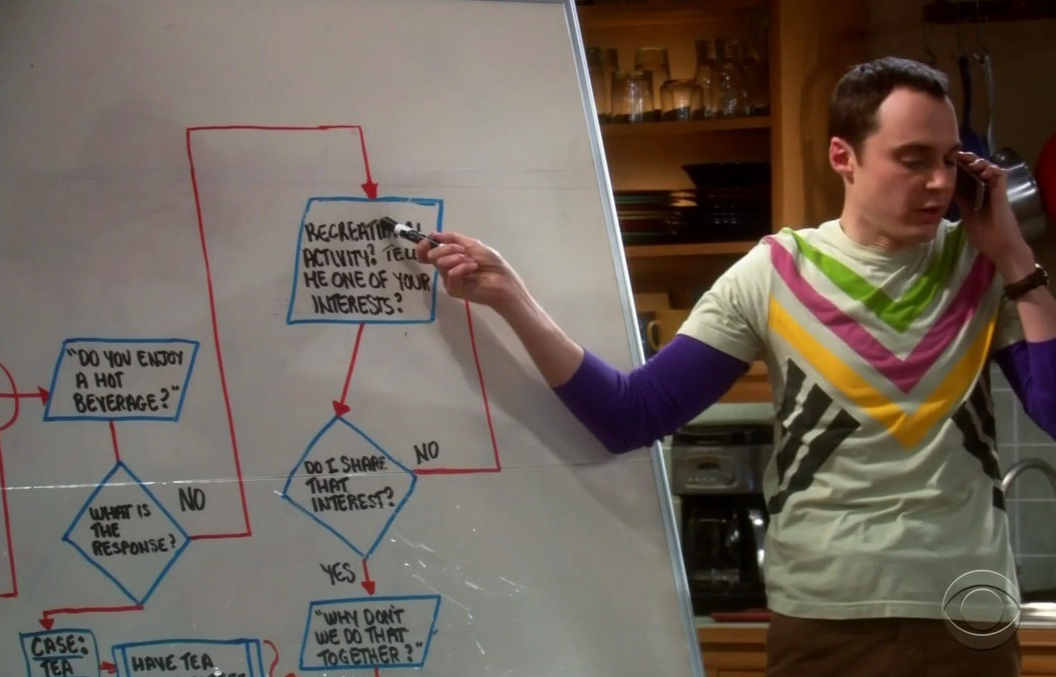
\includegraphics[width=7cm]{fig/Algorithm-sheldon.png}
            }
                 \textit{ I believe I've isolateblblblblblblsblbslbslbsl
            sblbslblsblsblblsblbs
            lbslblbslsb d the algorithm for making friends.}
     
            
            \small{
            \hfill Sheldon Cooper, 
            
            \hfill in \textit{The Big Band Theory}, Season 2, Episode 13
            }


    \end{columns}

\end{frame}


%%%%%%%%%%%%%%%%%%%%%
\subsection{Introduction}
    \begin{frame}
    \frametitle{Pourquoi faire appel � des algorithmes ?}
    Pour automatiser des t�ches
    
    Exemples :
    \begin{itemize}
    \item M�tier � tisser\\
    \item M�thode de calcul � la main d'une division\\
    \item Recette de cuisine\\
    \item ...\\
    \end{itemize}
    \end{frame}
 
 %%%%%%%%%%%%%%%%%
 
    \begin{frame}
    \frametitle{Qu'est-ce qu'un algorithme ?}
    \begin{block}{D�finition}
    Un algorithme est un ensemble 
    ordonn� d'instructions simples
permettant de r�soudre un probl�me.
    \end{block}
    \end{frame}
    
 %%%%%%%%%%%%%%%%%%
 \subsection{Construction d'un algorithme}
%%%%%%%%%%%%%%%%%%%    
\section{La machine de Turing}
%%%%%%%%%%%%%%%%%%%%
 
  
\begin{frame}[fragile]
\frametitle{Un peu d'histoire...}
\begin{codeblock}{Test}
\begin{codeC}
for (int i = 0 ; i < n ; i ++) {
    //a comment
    printf("%d",i);
    }
\end{codeC}
\end{codeblock}

\begin{termblock}{test 2}
\lstset{escapeinside={��}}
\begin{lstlisting}
�\textbf{>>}�./a.out
�\color{darkgray}{\texttt{  Hello World}}�
\end{lstlisting}
\end{termblock}

 \begin{block}{Bloc standard}
blablabla
\end{block}
\end{frame}


\begin{frame}[fragile]
\frametitle{essai}
\begin{columns}
\column{6cm}
\begin{block}

\begin{figure}
\begin{tikzpicture} [
    auto,
    decision/.style = { diamond, draw=blue, thick, fill=blue!20,
                        text width=5em, text badly centered,
                        inner sep=1pt, rounded corners },
    block/.style    = { rectangle, draw=blue, thick, 
                        fill=blue!20, text width=10em, text centered,
                        rounded corners, minimum height=2em },
    line/.style     = { draw, thick, ->, shorten >=2pt },
  ]
   \matrix [column sep=-10mm, row sep=10mm] {
                    & \node [text centered] (x) {$\mathbf{X}$};            & \\
                    & \node (null1) {};                                    & \\
                    & \node [block] (doa) {\textsf{DoAE}($\mathbf{X}$)};   & \\
  	               \node(null3){}; & \node [decision] (uiddes)
                        {\textsf{UID}($\hat{\mathbf{X}}$)};
                                  & \node[text centered](tra){$\mathbf{i}$}; \\
                  & \node [block] (track) {\textsf{DoAT}($\mathbf{x}$)}; & \\
                    & \node [block] (pesos)
                        {\textsf{BF}(DoA$_{\mathrm{T}}$,DoAs)};            & \\
                    & \node [block] (filtrado)
                        {\textsf{SF}($\mathbf{w}$,$\mathbf{x}$)};          & \\
                    & \node [text centered] (xf) {$\hat{x}(t)$ };          & \\
  };
  % connect all nodes defined above
 \begin{scope} [every path/.style=line]
    \path (x)        --    (doa);
    \path (doa)      --    node [near start] {DoAs} (uiddes);
    \path (tra)      --    (uiddes);
    \path (uiddes)   --++  (-3,0) node [near start] {no} |- (null1);
    \path (uiddes)   --    node [near start] {DoA} (track);
    \path (track)    --    node [near start] {DoA$_{\mathrm{T}}$} (pesos);
    \path (pesos)    --    node [near start] {\textbf{w}} (filtrado);
    \path (filtrado) --    (xf);
  
  \end{scope}
\end{tikzpicture}
\end{figure}
\end{block}
\column{3cm}
\begin{block}{bulbul}
\end{block}
\end{columns}
\end{frame}

\end{document}
